\documentclass{article}

\usepackage{opts}

\begin{document}

\listoffigures
\clearpage

\tikzsetnextfilename{kernel-block}
\begin{figure}
  \centering\resizebox{\textwidth}{!}{
    \begin{tikzpicture}[%
      node font=\humor,
      decoration={amplitude=1.5pt}, penciline={jag ratio=2},%
      every node/.style = {thick,decorate,align=center},%
      hw/.style = {draw,minimum width=10cm},%
      dev/.style = {draw,minimum width=0cm},%
      inproc/.style = {draw,minimum width=3cm},%
      arrow/.style = {<->,>=stealth,decorate}]      

  \node (hw) [hw] {Hardware};%
  \node (hwctrl) [hw,above=of hw] {Hardware control};%
  \node (drv) [draw,above=5mm of hwctrl.north west,anchor=south west,minimum width=4cm]%
  {Device drivers};%
  \node (chr) [dev,above=0pt of drv.north west,anchor=south west,scale=.95] {Character\\devices};%
  \node (blk) [dev,above=0pt of drv.north east,anchor=south east,minimum width=2cm,scale=.95]%
  {Block\\devices};%
  \node (buf) [draw,above=5mm of blk.north east,anchor=south east,minimum width=2cm] {Buffer\\cache};%

  \node (fs) [draw,above=5mm of buf.north east, anchor=south east,xshift=5mm,%
  minimum height=3cm,minimum width=4.5cm,%
  label={above,yshift=-4ex:{File subsystem}}] {};%
  \node (vfs)  [draw,below=7ex of fs.north,anchor=north,minimum width=3.5cm] {VFS};%
  \node (nfs)  [draw,below=3ex of vfs.south west,anchor=north west,scale=.6] {NFS};%
  \node (more) [draw,right=3mm of nfs,scale=.8] {$\cdots$};%
  \node (ext2) [draw,right=3mm of more,scale=.6] {Ext2};%
  \node (vfat) [draw,right=3mm of ext2,scale=.6] {VFAT};%

  \draw [arrow]  (nfs.north)-- ++ (0,5mm);%
  \draw [arrow] (more.north)-- ++ (0,5mm);%
  \draw [arrow] (ext2.north)-- ++ (0,5mm);%
  \draw [arrow] (vfat.north)-- ++ (0,5mm);%
  
  \node (proc) [draw,right=of fs.north east,anchor=north west,%
  minimum height=5.5cm,minimum width=4.5cm,%
  label={above,yshift=-6ex,align=center:{Process control\\subsystem}}] {};%
  \node (ipc) [inproc,below=9ex of proc.north, anchor=north] {Inter-process\\communication};%
  \node (sched) [inproc,below=2mm of ipc] {Scheduler};%
  \node (mm) [inproc,below=2mm of sched] {Memory\\management};%

  \node (syscall) [draw,above=7.7cm of hwctrl.north,anchor=south,%
  minimum width=8cm] {System call interface};%
  \node (lib) [draw,above=of syscall.north east,anchor=south east,minimum width=4cm]%
  {Libraries};%

  \draw [decorate,dashed] ($(hw.north west) + (0,5mm)$)--%
  node [above,xshift=-4.3cm,scale=.6] {Kernel level}%
  node [below,xshift=-4.15cm,scale=.6]{Hardware level}%
  ($(hw.north east) + (0,5mm)$);%

  \draw [decorate,dashed] ($(syscall.north west) + (-1cm,5mm)$)--%
  node [above,xshift=-4.45cm,scale=.6] {User level}%
  node [below,xshift=-4.3cm,scale=.6]{Kernel level}%
  ($(syscall.north east) + (1cm,5mm)$);%

  \node (user) [above=of lib.north west,anchor=east] {User programs};%

  \draw [arrow] (user.south east)--(lib.north);%
  \draw [arrow] (user.south)-- node [rotate=90,above,scale=.6] {trap} (user |- syscall.north);%
  \draw [arrow] (lib.south)--node [rotate=90,above,scale=.6] {trap} (lib |- syscall.north);%
  \draw [arrow] (fs.north) -- (fs |- syscall.south);%
  \draw [arrow] (proc.north) -- (proc |- syscall.south);%
  \draw [arrow] (ext2.south) -- (ext2 |- buf.north);%
  \draw [arrow] (vfat.south) -- (vfat |- buf.north);%
  \draw [arrow] (buf.south) -- (buf |- blk.north);%
  \draw [arrow] (nfs.south) -- (nfs |- chr.north);%
  \draw [arrow] (drv.south) -- (drv |- hwctrl.north);%
  \draw [arrow] (proc.south) -- (proc |- hwctrl.north);%
  \draw [arrow] (hwctrl) -- (hw);
  \draw [arrow] (fs.east) -- (fs -| proc.west);%
\end{tikzpicture}}
  \caption{OS overview}
  \label{fig:kernel-block}
\end{figure}

\tikzsetnextfilename{chipsets}
\begin{figure}
  \centering
  \begin{tikzpicture}[node font=\humor,node distance=0pt,%
    decoration={amplitude=1pt}, penciline={jag ratio=1}, thick]%
  
    \tikzset{%
      every node/.style ={draw,decorate,align=center},
      squarebox/.style = {%      
        fill=blue!30,minimum width=2cm,inner sep=1pt},%
      varrow/.style = {%
        double arrow,rotate=90,scale=.7,fill=gray!30,draw,%
        double arrow tip angle=135,%
        double arrow head extend=6pt},%
      harrow/.style = {%
        double arrow,fill=gray!30,draw,scale=.7,%
        inner xsep=.5cm,%
        double arrow head extend=3pt}}  

  \node (cpu) [squarebox,fill=red!30] {Intel Core 2\\(CPU)};%
  \node (fsb) [varrow,below=of cpu.south,anchor=east] {Front\\Side\\Bus};
  \node (nb)  [squarebox,below=of fsb.west,fill=orange!30] {North bridge\\Chip};
  \node (ddr2) [harrow,left=of nb.west,anchor=east,scale=.6] {DDR2};
  \node (ram) [squarebox,left=of ddr2.west,anchor=east] {System RAM};
  \node (a4) [harrow,right=of nb.east,anchor=west] {};
  \node (gpu) [squarebox,right=of a4.east,anchor=west] {Graphics Card};
  \node (dmi) [varrow,below=of nb.south,anchor=east] {DMI\\Interface};
  \node (sb)  [squarebox,below=of dmi.west,fill=orange!30] {South bridge\\Chip};
  \node (a5) [harrow,left=of sb.west,anchor=east] {};
  \node (ata) [squarebox,left=of a5.west] {Serial ATA Ports};
  \node (a6) [harrow,right=of sb.east,anchor=west] {};
  \node (clock) [squarebox,right=of a6.east,anchor=west] {Clock Generation};
  \node (bios) [squarebox,above=2mm of ata.north east,anchor=south east] {BIOS};
  \node (usb) [squarebox,below=2mm of ata.south east,anchor=north east] {USB Ports};
  \node (power) [squarebox,above=2mm of clock.north west,anchor=south west] {Power Management};
  \node (pci) [squarebox,below=2mm of clock.south west,anchor=north west] {PCI Bus};
  \node (a7) [harrow,above=10pt of a5.north,anchor=south,rotate=160,inner xsep=.6cm,xshift=-2pt] {};
  \node (a8) [harrow,below=5pt of a5.south,anchor=north,rotate=20,inner xsep=.6cm,xshift=0pt] {};
  \node (a9) [harrow,above=5pt of a6.north,anchor=south,rotate=20,inner xsep=.6cm,xshift=0pt] {};
  \node (a10) [harrow,below=10pt of a6.south,anchor=north,rotate=160,inner xsep=.6cm,xshift=2pt] {};
\end{tikzpicture}  
  \caption{Motherboard chipsets}
  \label{fig:chipsets}
\end{figure}

\tikzsetnextfilename{chipsets-bw}
\begin{figure}
  \centering
  \begin{tikzpicture}[ node distance=0pt, node font=\humor,%
    decoration={amplitude=1pt}, penciline={jag ratio=1}, thick]
  
    \tikzset{%
      every node/.style = {draw,decorate,align=center},%
      squarebox/.style = {minimum width=2cm,inner sep=1pt},%
      varrow/.style = {%
        double arrow,rotate=90,scale=.7,%
        double arrow tip angle=135,%
        double arrow head extend=6pt},%
      harrow/.style = {inner xsep=.5cm,%
        double arrow,scale=.7,%
        double arrow head extend=3pt}}%

    \node (cpu) [squarebox] {Intel Core 2\\(CPU)};%
    \node (fsb) [varrow,below=of cpu.south,anchor=east] {Front\\Side\\Bus};%
    \node (nb) [squarebox,below=of fsb.west] {North bridge\\Chip};%
    \node (ddr2) [harrow,left=of nb.west,anchor=east,scale=.6] {DDR2};%
    \node (ram) [squarebox,left=of ddr2.west,anchor=east] {System RAM};%
    \node (a4) [harrow,right=of nb.east,anchor=west] {};%
    \node (gpu) [squarebox,right=of a4.east,anchor=west] {Graphics Card};%
    \node (dmi) [varrow,below=of nb.south,anchor=east] {DMI\\Interface};%
    \node (sb) [squarebox,below=of dmi.west] {South bridge\\Chip};%
    \node (a5) [harrow,left=of sb.west,anchor=east] {};%
    \node (ata) [squarebox,left=of a5.west] {Serial ATA Ports};%
    \node (a6) [harrow,right=of sb.east,anchor=west] {};%
    \node (clock) [squarebox,right=of a6.east,anchor=west] {Clock Generation};%
    \node (bios) [squarebox,above=2mm of ata.north east,anchor=south east] {BIOS};%
    \node (usb) [squarebox,below=2mm of ata.south east,anchor=north east] {USB Ports};%
    \node (power) [squarebox,above=2mm of clock.north west,anchor=south west] {Power
      Management};%
    \node (pci) [squarebox,below=2mm of clock.south west,anchor=north west] {PCI Bus};%
    \node (a7) [harrow,above=10pt of a5.north,anchor=south,rotate=160,inner
    xsep=.6cm,xshift=-2pt] {};%
    \node (a8) [harrow,below=5pt of a5.south,anchor=north,rotate=20,inner
    xsep=.6cm,xshift=0pt] {};%
    \node (a9) [harrow,above=5pt of a6.north,anchor=south,rotate=20,inner
    xsep=.6cm,xshift=0pt] {};%
    \node (a10) [harrow,below=10pt of a6.south,anchor=north,rotate=160,inner
    xsep=.6cm,xshift=2pt] {};%
  \end{tikzpicture}
  \caption{Motherboard chipsets (bw version)}
  \label{fig:chipsets-bw}
\end{figure}

\tikzsetnextfilename{mos-figs-1-6}
\begin{figure}
  \centering
\begin{tikzpicture}[node font=\humor,ultra thick,node distance=0pt,%
  decoration=bent,
  every node/.style = {draw,align=center},%
  arrow/.style = {single arrow,inner xsep=3mm, single arrow head extend=3pt},
  start chain]%
  
  \node [on chain,decorate] (fetch) {Fetch\\unit};%
  \node [on chain] (f2d) [arrow] {};%
  \node [on chain,decorate] (decode) {Decode\\unit};%
  \node [on chain] (d2e) [arrow] {};%
  \node [on chain,decorate] (exec) {Execute\\unit};%
\end{tikzpicture}  
  \caption{CPU's working cycle}
  \label{fig:mos-figs-1-6}
\end{figure}

\tikzsetnextfilename{boot}
\begin{figure}
  \centering\resizebox{\textwidth}{!}{
    \begin{tikzpicture}[decoration={amplitude=2pt}, penciline={jag ratio=2},%
      node font=\humor,thick,%
      arrow/.style = {decorate,->},%
      every join/.style = {decorate,->},%
      every node/.style = {decorate,draw,align=center},%
      squarebox/.style = {fill=blue!20,minimum width=70pt,minimum height=40pt},%
      longbox/.style = {inner sep=5pt},%
      dashframe/.style = {dashed,gray!30,minimum height=150pt}]%

      {[start chain] %
        \node [on chain,join,squarebox] (biosinit) {BIOS\\Initialization};%
        \node [on chain,join,squarebox] (mbr) {MBR};%
        \node [on chain,join,squarebox] (bootldr) {Boot Loader};%
        \node [on chain,join,squarebox] (kinit1) {Earily\\Kernel\\Initialization};%
        \node [on chain,join,squarebox] (kinit2) {Full\\Kernel\\Initialization};%
        \node [on chain,join,squarebox] (user) {First\\User Mode\\Process};%
      }%

      \node (biosserv) [longbox,below=1cm of mbr.south west,anchor=north west,%
      minimum width=275pt, fill=orange!30] {BIOS Services};%
      \node (kserv) [longbox,below=1cm of user.south east,anchor=north east,%
      fill=red!30] {Kernel Services};%
      \node (hw) [longbox,below=0pt of kserv.south east,anchor=north east, yshift=2pt,%
      minimum width=580pt,fill=gray!50] {Hardware};%

      \draw [arrow] (biosinit.south)--(biosinit |- hw.north);%
      \draw [arrow] (mbr.south)--(mbr |- biosserv.north);%
      \draw [arrow] (bootldr.south)--(bootldr |- biosserv.north);%
      \draw [arrow] (kinit1.south)--(kinit1 |- biosserv.north);%
      \draw [arrow] (kinit2.south)--(kinit2 |- hw.north);%
      \draw [arrow] (user.south)--(user |- kserv.north);%

      \node (real) [dashframe,minimum width=395pt,below=10pt of hw.south west,%
      anchor=south west,xshift=-6pt] {};%
      \node (protected) [dashframe,minimum width=187pt,right=10pt of
      real.east,anchor=west] {};%

      \node (frm1) [draw=none,right=0pt of real.north west, anchor=north west] {CPU in Real Mode};%
      \draw [arrow] ($(frm1.north west) + (0,10pt)$) to node [above,draw=none] {Time flow}%
      ($(frm1.north east) + (0,10pt)$);%
      \node (frm2) [right=0pt of protected.north west, anchor=north west,draw=none]%
      {CPU in Protected Mode};%
      \node (switch) [above=10pt of protected.north west, anchor=south west,%
      xshift=-5pt,align=left,scale=.6,gray!90,draw=none] {Switch to\\Protected Mode};%
      \draw [arrow,>=stealth,thin,gray!90] (switch.south west)--(kinit1.east);
    \end{tikzpicture}}
  \caption{Bootstrapping}
  \label{fig:boot}
\end{figure}

\tikzsetnextfilename{boot-bw}
\begin{figure}
  \centering\resizebox{\textwidth}{!}{
    \begin{tikzpicture}[decoration={amplitude=2pt}, penciline={jag ratio=2},%
      node font=\humor,thick,%
      arrow/.style = {decorate,->},%
      every edge/.style = {decorate,<-,draw},%
      every node/.style = {decorate,draw,align=center},%
      squarebox/.style = {minimum width=70pt,minimum height=40pt},%
      longbox/.style = {inner sep=5pt},%
      dashframe/.style = {dashed,minimum height=150pt}]%

      {[start chain] %
        \node [on chain,squarebox] (biosinit) {BIOS\\Initialization};%
        \node [on chain,squarebox] (mbr) {MBR} edge (biosinit);%
        \node [on chain,squarebox] (bootldr) {Boot Loader} edge (mbr);%
        \node [on chain,squarebox] (kinit1) {Earily\\Kernel\\Initialization} edge (bootldr); %
        \node [on chain,squarebox] (kinit2) {Full\\Kernel\\Initialization} edge (kinit1);%
        \node [on chain,squarebox] (user) {First\\User Mode\\Process} edge (kinit2);%
      }%

      \node (biosserv) [longbox,below=1cm of mbr.south west,anchor=north west,%
      minimum width=275pt] {BIOS Services};%
      \node (kserv) [longbox,below=1cm of user.south east,anchor=north east]
      {Kernel Services};%      
      \node (hw) [longbox,below=0pt of kserv.south east,anchor=north east, yshift=2pt,%
      minimum width=580pt] {Hardware};%

      \draw [arrow] (biosinit.south)--(biosinit |- hw.north);%
      \draw [arrow] (mbr.south)--(mbr |- biosserv.north);%
      \draw [arrow] (bootldr.south)--(bootldr |- biosserv.north);%
      \draw [arrow] (kinit1.south)--(kinit1 |- biosserv.north);%
      \draw [arrow] (kinit2.south)--(kinit2 |- hw.north);%
      \draw [arrow] (user.south)--(user |- kserv.north);%

      \node (real) [dashframe,minimum width=395pt,below=10pt of hw.south west,%
      anchor=south west,xshift=-6pt] {};%
      \node (protected) [dashframe,minimum width=187pt,right=10pt of
      real.east,anchor=west] {};%

      \node (frm1) [draw=none,right=0pt of real.north west, anchor=north west] {CPU in Real Mode};%
      \draw [arrow] ($(frm1.north west) + (0,10pt)$) to node [above,draw=none] {Time flow}%
      ($(frm1.north east) + (0,10pt)$);%
      \node (frm2) [right=0pt of protected.north west, anchor=north west,draw=none]%
      {CPU in Protected Mode};%
      \node (switch) [above=10pt of protected.north west, anchor=south west,%
      xshift=-5pt,align=left,scale=.6,draw=none] {Switch to\\Protected Mode};%
      \draw [arrow,>=stealth,thin] (switch.south west)--(kinit1.east);
    \end{tikzpicture}}
  \caption{Bootstrapping (bw version)}
  \label{fig:boot-bw}
\end{figure}

\tikzsetnextfilename{mos-figs-1-20}
\begin{figure}
  \centering\resizebox{.5\textwidth}{!}{
\begin{tikzpicture}[node distance=0pt,inner sep=0pt,ultra thick,%
  decoration={amplitude=2pt}, penciline={jag ratio=2},%
  every text node part/.style = {align=center},%
  arrow/.style = {decorate,->},%
  node font=\humor
  ]

  \node [name=proc,%
  rectangle split,rectangle split parts=4,rectangle split empty part height=2cm,%
  draw,decorate,%
  inner ysep=3pt,minimum width=2cm,%
  ] {%
    Stack%
    \nodepart{two}%
    \nodepart{three} Data%
    \nodepart{four} Text%
  };%

  \node [right=of proc.south east,anchor=south west] {0000};%
  \node [right=of proc.north east,anchor=north west] {FFFF};%
  
  \node (gap) [above=of proc.two split,anchor=south,%
  minimum width=1.9cm,minimum height=2.2cm,%
  decorate,pattern=north east lines,pattern color=gray!30] {gap};%
  \draw [arrow] ($(gap.south) + (.5cm,0)$)-- +(0,5mm);%
  \draw [arrow] ($(gap.north) + (.5cm,0)$)-- +(0,-5mm);%

\end{tikzpicture}}
  \caption{Process' virtual address space}
  \label{fig:mos-figs-1-20}
\end{figure}

\tikzsetnextfilename{mm-process}
\begin{figure}
  \centering\resizebox{.5\textwidth}{!}{
\begin{tikzpicture}
  \begin{pgfonlayer}{background}
    \node [inner sep=0] at (current page.center) {%
      \includegraphics[width=\paperwidth]{memory1}
    };
  \end{pgfonlayer}
  \node at (current page.south) [yshift=2cm,scale=3,align=center]%
  {\humor{the size of a process}\\\humor{(text + data + bss) is}\\\humor{established at compile time}};
\end{tikzpicture}}
  \caption{UNIX view of a process}
  \label{fig:mm-process}
\end{figure}

\tikzsetnextfilename{process-creation}
\begin{figure}
  \centering\resizebox{.5\textwidth}{!} {
\begin{tikzpicture}[ decoration={amplitude=1pt}, penciline={jag ratio=1},%
  node distance=5mm, ultra thick,font=\purisa, %
  every node/.style ={inner sep=2pt},%
  every edge/.style ={draw,gray!80,decorate,->},%
  every edge quotes/.style ={font=\purisa\tiny,sloped,auto}%
  ]%
  \node (exit) {exit()};%
  \node (exec) [left=of exit] {exec()};%
  \node (fork) [above left=of exec, xshift=15pt] {fork()};%
  \node (wait) [above right=of exit, xshift=-15pt] {wait()};%
  \node (any)  [above right=of fork, xshift=-6pt] {anything()};%

  \path
  (fork) edge ["parent" near end,bend left] (any.west)%
  (any.east)  edge [bend left] (wait)%
  (fork) edge ["child"' near end,bend right] (exec)%
  (exec) edge  (exit)%
  (exit) edge [bend right] (wait);%
\end{tikzpicture} }
  \caption{Process creation}
  \label{fig:process-creation}
\end{figure}

\tikzsetnextfilename{thread-operations}
\begin{figure}
  \centering\resizebox{.5\textwidth}{!}{
\begin{tikzpicture}[auto, decoration={amplitude=1.5pt}, penciline={jag ratio=2}]%
  \tikzset{%
    main node/.style = {decorate,draw,ultra thick,inner sep=2pt,scale=1.5,%
      node distance=10em,align=center,% text width=5em,text centered,minimum size=4mm,
    },%
    every edge/.style = {draw,decorate,ultra thick,->},%
    every edge quotes/.style={opacity=.9,font=\purisa\footnotesize}
  }
  
  \node [main node,circle] (start) {Start\\with one\\thread\\running};
  \node [main node] (t1) [above right=of start] {thread1};
  \node [main node] (t2)       [right=of start] {thread2};
  \node [main node] (t3) [below right=of start] {thread3};
  \node [main node,circle] (end) [right=of t2] {end};
  \node [main node] (yield) [right=of t1] {release\\CPU};
  \node [main node] (join) [right=of t3] {wait for\\a thread\\to exit};
  \path%
  (start.north) edge ["thread\_create()" near end,sloped,bend left=10,] (t1.west)%
  (start.south) edge ["thread\_create()"' near end,sloped,bend right=10,rotate=7] (t3.west)%
  (start) edge ["thread\_create()"] (t2)%
  (t1) edge ["thread\_exit()"' near end,sloped,bend left=20,rotate=-6] (end)%
  edge ["thread\_yield()"] (yield)%
  (t3) edge ["thread\_exit()"  near end,sloped,bend right=20,rotate=4] (end)%
  edge ["thread\_join()"'] (join)%
  (t2) edge ["thread\_exit()"] (end);%
\end{tikzpicture}}
  \caption{Thread operations}
  \label{fig:thread-operations}
\end{figure}

\tikzsetnextfilename{deadlock-resource}
\begin{figure}
  \centering\resizebox{.6\textwidth}{!}{
\begin{tikzpicture}[every node/.style = {inner sep=0}]
  %%% background image
  \node[anchor=south west] (image) at (0,0)%
  {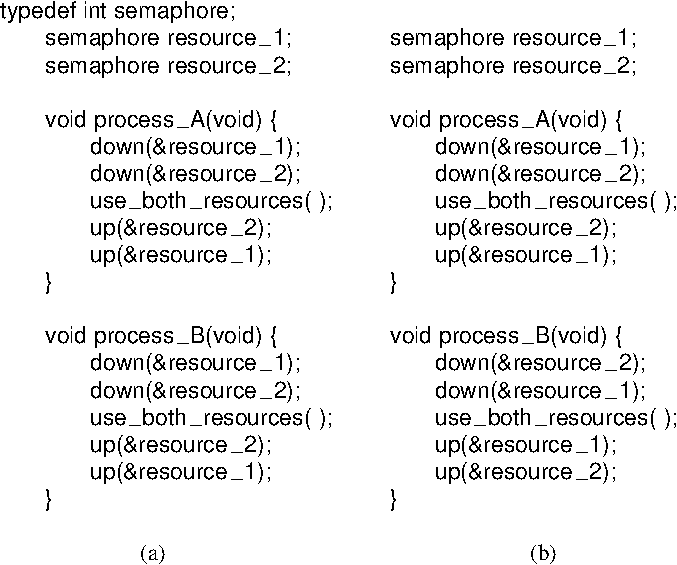
\includegraphics[width=\paperwidth]{mos-figs-3-2}};

  % http://tex.stackexchange.com/questions/9559/drawing-on-an-image-with-tikz
  \begin{scope}[x={(image.south east)},y={(image.north west)}]%
    % %%% grid
    % \draw[help lines,xstep=.1,ystep=.1] (0,0) grid (1,1);%
    % \foreach \x in {0,1,...,9} { \node [xy,anchor=north] at (\x/10,0) {0.\x}; }%
    % \foreach \y in {0,1,...,9} { \node [xy,anchor=east] at (0,\y/10) {0.\y}; }%

    \node [opacity=0.4,color=red,scale=6,rotate=45] at
    (.6,.3) [anchor=west] {Deadlock!};
  \end{scope}
\end{tikzpicture}}
  \caption{Deadlock --- Resource issues}
  \label{fig:deadlock-resource}
\end{figure}
  
\tikzsetnextfilename{deadlock-graph}
\begin{figure}
  \centering\resizebox{.6\textwidth}{!}{
    \begin{tikzpicture}[%
      r/.style={rectangle, draw,thick},
      p/.style={circle, draw, thick},
      every edge quotes/.style={auto=right,font=\footnotesize},
      every label quotes/.style={below},
      every edge/.style={draw,->, >=stealth, thick}]

      \node (a) [p] {A};
      \node (r) [r, below=of a] {R} edge ["has"](a);
      \node (s) [r, right=of a] {S};
      \node (b) [p, below=of s] {B} edge ["wants"](s);

      \node (d) [p, right=2.7cm of s,yshift=6mm] {D};
      \node (u) [r, below right=of d] {U} edge [bend right, <-] (d);
      \node (c) [p, below  left=of u] {C} edge [bend right, <-] (u);
      \node (t) [r, below  left=of d] {T} edge [bend right, <-] (c) edge [bend left] (d);
\end{tikzpicture}}
  \caption{Deadlock notions}
  \label{fig:deadlock-graph}
\end{figure}

\tikzsetnextfilename{deadlock-banker}
\begin{figure}
  \centering\resizebox{\textwidth}{!}{
\begin{tikzpicture}
  %%% background image
  \node[anchor=south west,inner sep=0] (image) at (0,0)%
  {\includegraphics[width=\paperwidth]{mos-figs-3-11}};

  % http://tex.stackexchange.com/questions/9559/drawing-on-an-image-with-tikz
  \begin{scope}[x={(image.south east)},y={(image.north west)}]%
    % %%% grid
    % \draw[help lines,xstep=.1,ystep=.1] (0,0) grid (1,1);%
    % \foreach \x in {0,1,...,9} { \node [xy,anchor=north] at (\x/10,0) {0.\x}; }%
    % \foreach \y in {0,1,...,9} { \node [xy,anchor=east] at (0,\y/10) {0.\y}; }%

    \node [inner sep=0,color=red,opacity=.3]%
    at (.81,.45) [anchor=west,rotate=30,scale=3.2] {unsafe!};
    \end{scope}
\end{tikzpicture}}
  \caption{Deadlock --- Banker algorithm}
  \label{fig:deadlock-banker}
\end{figure}

\tikzsetnextfilename{deadlock-avoidance}
\begin{figure}
  \centering\resizebox{\textwidth}{!}{
\begin{tikzpicture}[
  text node/.style={inner sep=0mm,color=blue!70,opacity=.7,scale=4.5,rotate=15},%
  ]
  %%% background image
  \node[anchor=south west,inner sep=0] (image) at (0,0)%
  {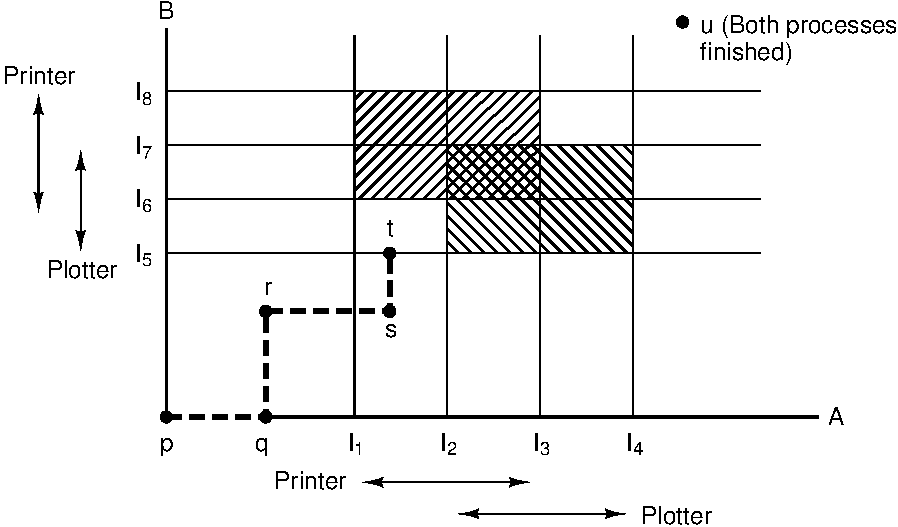
\includegraphics[width=\paperwidth]{mos-figs-3-8}};

  % http://tex.stackexchange.com/questions/9559/drawing-on-an-image-with-tikz
  \begin{scope}[x={(image.south east)},y={(image.north west)}]%
    % %%% grid
    % \draw[help lines,xstep=.1,ystep=.1] (0,0) grid (1,1);%
    % \foreach \x in {0,1,...,9} { \node [xy,anchor=north] at (\x/10,0) {0.\x}; }%
    % \foreach \y in {0,1,...,9} { \node [xy,anchor=east] at (0,\y/10) {0.\y}; }%

    \node [text node] at (.5,.73) {dead};%
    \node [text node] at (.6,.61) {zone};%

    \draw [fill=red!70,opacity=.3]%
    (.395,.52) -- (.395,.62) -- (.499,.62) -- (.499,.52) -- cycle;%

    \node (anno) [color=red,rounded corners,draw] at (.6,.35) {Unsafe region};%
    \draw [->,very thick,color=red!40,] (anno.west) to [bend left] (.48,.52);%

    \draw [fill=gray!50,opacity=.2] (.5,.52) -- (.705,.52) -- (.705,.825) -- (.395,.825)
    -- (.395,.62) -- (.5,.62) -- cycle;
  \end{scope}
\end{tikzpicture}}  
  \caption{Deadlock avoidance}
  \label{fig:deadlock-avoidance}
\end{figure}

\tikzsetnextfilename{deadlock-avoidance-2}
\begin{figure}
  \centering\resizebox{\textwidth}{!}{
\begin{tikzpicture}[every node/.style = {inner sep=0}]
  %%% background image
  \node[anchor=south west] (image) at (0,0)%
  {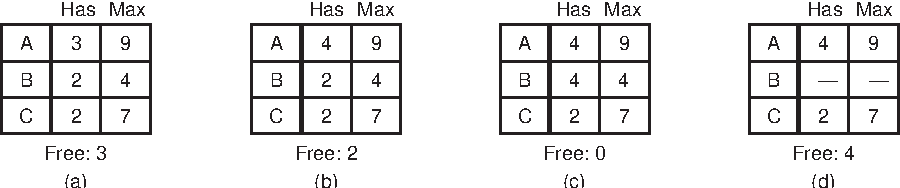
\includegraphics[width=\paperwidth]{mos-figs-3-10}};

  % http://tex.stackexchange.com/questions/9559/drawing-on-an-image-with-tikz
  \begin{scope}[x={(image.south east)},y={(image.north west)}]%
    % %%% grid
    % \draw[help lines,xstep=.1,ystep=.1] (0,0) grid (1,1);%
    % \foreach \x in {0,1,...,9} { \node [xy,anchor=north] at (\x/10,0) {0.\x}; }%
    % \foreach \y in {0,1,...,9} { \node [xy,anchor=east] at (0,\y/10) {0.\y}; }%
    
    \node at (.365,.55) [color=red,text opacity=.3,scale=2.5,rotate=15] {unsafe};%
  \end{scope}
\end{tikzpicture}}
  \caption{Deadlock avoidance}
  \label{fig:deadlock-avoidance-2}
\end{figure}

\tikzsetnextfilename{ipc}
\begin{figure}
  \centering\resizebox{.6\textwidth}{!}{
\begin{tikzpicture}[auto,node distance=0pt,%
  textnode/.style ={circle,fill=blue!20,align=center,inner sep=1pt,minimum size=4mm,draw},%
  arrow/.style = {single arrow,single arrow head indent=1ex,%
    align=center,scale=.6,draw,fill=orange!30}] 
  
  {[start chain]%
    \node [on chain, textnode] (compiler) {compiler};%
    \node [on chain, arrow] (asm) {Assembly\\code};%
    \node [on chain, textnode] (assembler) {assembler};%
    \node [on chain, arrow] (obj) {Object\\module};%
    \node [on chain, textnode] (loader) {loader};%
  }

  {[start chain]%
    \node [on chain, textnode] (print) [above=1cm of asm] {Process\\wants\\printing};%
    \node [on chain, arrow, draw] (file) {{\Large file}};%
    \node [on chain, textnode] (printer) {Printer\\daemon};%
  }
\end{tikzpicture}}
\caption{Producers and consumers}
  \label{fig:ipc}
\end{figure}

\tikzsetnextfilename{ipc-bw}
\begin{figure}
  \centering\resizebox{.6\textwidth}{!}{
\begin{tikzpicture}[auto,node distance=0pt,%
  textnode/.style ={circle,align=center,inner sep=1pt,minimum size=4mm,draw},%
  arrow/.style = {single arrow,single arrow head indent=1ex,align=center,scale=.6,draw}]   

  {[start chain]%
    \node [on chain, textnode] (compiler) {compiler};%
    \node [on chain, arrow] (asm) {Assembly\\code};%
    \node [on chain, textnode] (assembler) {assembler};%
    \node [on chain, arrow] (obj) {Object\\module};%
    \node [on chain, textnode] (loader) {loader};%
  }
  {[start chain]%
    \node [on chain, textnode] (print) [above=1cm of asm] {Process\\wants\\printing};%
    \node [on chain, arrow, draw] (file) {{\Large file}};%
    \node [on chain, textnode] (printer) {Printer\\daemon};%
  }  
\end{tikzpicture}}
  \caption{Producers and consumers (bw version)}
  \label{fig:ipc-bw}
\end{figure}

\tikzsetnextfilename{circular}
\begin{figure}
  \centering\resizebox{.5\textwidth}{!}{
    \begin{tikzpicture} [%
      every node/.style = {circle,font=\fontspec{Humor Sans},minimum width=28pt},
      % pinnode/.style = {circle,minimum width=25pt},%
      every pin/.style = {minimum size=0pt, pin distance=1mm, inner sep=1pt,%
        pin edge={gray!50,thick,dashed}}]%
  
  {[start chain=circle placed {at =(\tikzchaincount*45:1.3)}]
    \foreach \n in {1,...,8} \node (N\n) [on chain,fill=gray!30] {};
  }
  
  \foreach \angle/\label in {0/c, 45/b, 90/a}%
  \node [fill=blue!40] (N\angle) at (\angle:1.3) {\LARGE\label};%

  \node [pin=270:{\tiny out}] at (90:1.3) {};%
  \node [pin=135:{\tiny in}] at (315:1.3) {};%

\end{tikzpicture}}
  \caption{A circular array}
  \label{fig:circular}
\end{figure}

\tikzsetnextfilename{circular-bw}
\begin{figure}
  \centering\resizebox{.5\textwidth}{!}{
    \begin{tikzpicture} [%
      every node/.style = {circle,font=\fontspec{Humor Sans},minimum width=28pt},
      % pinnode/.style = {circle,minimum width=25pt},%
      every pin/.style = {minimum size=0pt, pin distance=1mm, inner sep=1pt,%
        pin edge={gray!50,thick,dashed}}]%
  
  {[start chain=circle placed {at =(\tikzchaincount*45:1.3)}]
    \foreach \n in {1,...,8} \node (N\n) [on chain,draw] {};
  }
  
  \foreach \angle/\label in {0/c, 45/b, 90/a}%
  \node (N\angle) at (\angle:1.3) {\LARGE\label};%

  \node [pin=270:{\tiny out}] at (90:1.3) {};%
  \node [pin=135:{\tiny in}] at (315:1.3) {};%

\end{tikzpicture}}
  \caption{A circular array (bw version)}
  \label{fig:circular-bw}
\end{figure}

\tikzsetnextfilename{mm-realmode}
\begin{figure}
  \centering\resizebox{\textwidth}{!}{
\begin{tikzpicture}
  %%% background image
  \node[anchor=south west,inner sep=0] (image) at (0,0)%
  {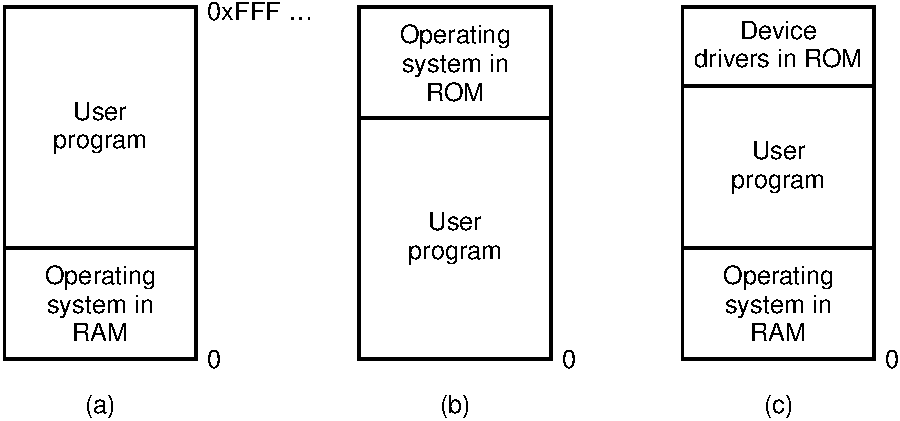
\includegraphics[width=\paperwidth]{mos-figs-4-1}};

  % http://tex.stackexchange.com/questions/9559/drawing-on-an-image-with-tikz
  \begin{scope}[x={(image.south east)},y={(image.north west)}]%
    % %%% grid
    % \draw[help lines,xstep=.1,ystep=.1] (0,0) grid (1,1);%
    % \foreach \x in {0,1,...,9} { \node [xy,anchor=north] at (\x/10,0) {0.\x}; }%
    % \foreach \y in {0,1,...,9} { \node [xy,anchor=east] at (0,\y/10) {0.\y}; }%

    \node at (.12,.1) {old mainstream};%
    \node at (.52,.1) {handhold, embedded};%
    \node at (.86,.1) {MS-DOS};%
  \end{scope}
\end{tikzpicture}}
  \caption{Real mode memory layouts}
  \label{fig:mm-realmode}
\end{figure}

\tikzsetnextfilename{tool-chain}
\begin{figure}
  \centering
  \begin{tikzpicture}[auto,%
    % decoration={random steps,segment length=7pt,amplitude=.7pt},
    tool/.style = {draw,decorate,align=center,fill=orange!20,ellipse},
    file/.style = {draw,decorate,align=center,fill=blue!10,rectangle},
    line/.style = {draw,decorate,thick, -latex', shorten >=2pt},
    every label/.style = {font=\ttfamily}]

    \matrix [row sep=5mm]%column sep=-1cm, 
    {
      % \node (emacs)[tool,%
      % %label={
\includegraphics[scale=.5]{programmer}},%
      % label={0:\textdollar{} emacs hello.c}] {Editor\\(\texttt{emacs})};\\%
      \node (hello-c) [file] {C source code\\(\texttt{hello.c})};\\%
      \node (cpp) [tool,label={0:\begin{tabular}{l}
          \$ cpp hello.c\\
          \$ gcc -E hello.c
        \end{tabular}}] {C Preprocessor\\(\texttt{cpp})};\\%
      \node (helloext) [file] {Extended C source code\\(\texttt{hello.i})};\\%
      \node (gcc) [tool,label={0:\begin{tabular}{l}
          \textdollar{} cc1 hello.i -o hello.s\\
          \textdollar{} gcc -S hello.c
        \end{tabular}}] {Compiler\\(\texttt{gcc})};\\%
      \node (hello-s) [file] {ASM source code\\(\texttt{hello.s})};\\%
      \node (as) [tool,label={0:\begin{tabular}{l}
          \textdollar{} as hello.s -o hello.o\\
          \textdollar{} gcc -c hello.c
        \end{tabular}}] {Assembler\\(\texttt{as})};\\%
      \node (hello-o) [file] {Object code\\(\texttt{hello.o})};\\%
      \node (ld) [tool,label={0:\begin{tabular}{l}
          \$ ld hello.o LIBs\\
          \$ gcc -o hello hello.c
        \end{tabular}}] {Linker\\(\texttt{ld})};\\%
      \node (hello) [file] {Executable program\\(\texttt{hello})};\\%
      % \node (gdb) [tool,label={0:\begin{tabular}{l}
      %   \$ gcc -g hello.c -o hello\\
      %   \$ gdb hello
      % \end{tabular}}] {Debugger\\(\texttt{gdb})};\\%
  };
 \node (stdio-h) [right=2mm of hello-c,file] {Include files, macros\\(\texttt{e.g. stdio.h})};%
 \node (printf) [right=2mm of hello-o,file] {Libraries\\(\texttt{e.g. printf})};

  \begin{scope}[every path/.style=line]
    % \path (emacs) -- (hello-c);
    \path (hello-c) -- (cpp);
    \path (stdio-h) -- (cpp);
    \path (cpp) -- (helloext);
    \path (helloext) -- (gcc);
    \path (gcc) -- (hello-s);
    \path (hello-s) -- (as);
    \path (as) -- (hello-o);
    \path (hello-o) -- (ld);
    \path (printf) -- (ld);
    \path (ld) -- (hello);
    % \path (hello) -- (gdb);
  \end{scope}
  \begin{scope}[every path/.style={decorate,decoration={brace,amplitude=10pt,mirror,raise=4pt}}]
      \draw ($(gcc.north west)+(-5mm,0)$) -- ($(as.south west)+(-5mm,0)$)%
      node [black,midway,xshift=-2cm,align=center] {Compile\\time};

      \draw [decoration={amplitude=5pt}]%
      ($(ld.north west)+(-3mm,0)$) -- ($(ld.south west)+(-3mm,0)$)%
      node [black,midway,xshift=-1.3cm,align=center] {Load\\time};

      \draw [decoration={amplitude=5pt}]%
      ($(hello.north west)+(-1mm,0)$) -- ($(hello.south west)+(-1mm,0)$)%
      node [black,midway,xshift=-1.2cm,align=center] {Run\\time};
  \end{scope}
\end{tikzpicture}
  \caption{Tool chain}
  \label{fig:tool-chain}
\end{figure}

\tikzsetnextfilename{mm-relocation}
\begin{figure}
  \centering\resizebox{\textwidth}{!}{
\begin{tikzpicture}[decoration={amplitude=2pt}, penciline={jag ratio=2},%
  textnode/.style = {inner sep=0pt,align=center,scale=3},%
  red line/.style = {decorate,->,opacity=.6,ultra thick,color=red!60},%
  blue line/.style = {decorate,->,opacity=.6,ultra thick,color=blue!60},%
  ]%
  %%% background image
  \node[anchor=south west,inner sep=0] (image) at (0,0)%
  {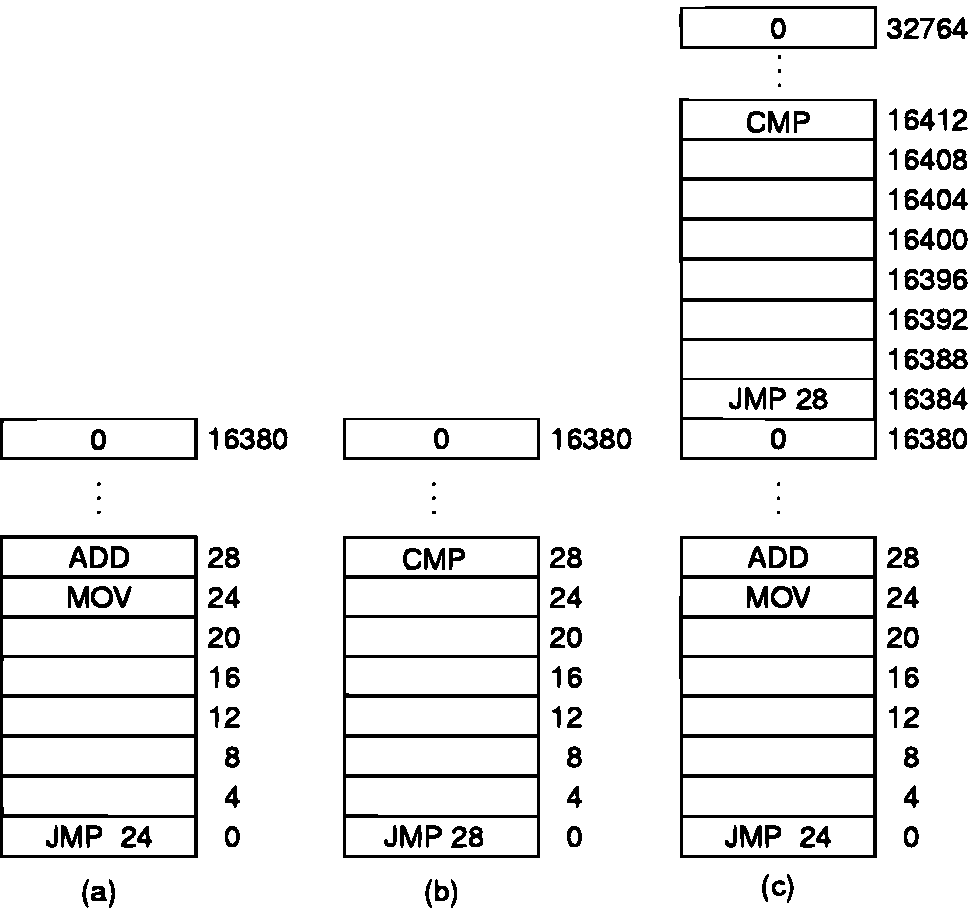
\includegraphics[width=\paperwidth]{relocation}};

  % http://tex.stackexchange.com/questions/9559/drawing-on-an-image-with-tikz
  \begin{scope}[x={(image.south east)},y={(image.north west)}]%
    %%% grid
    % \draw[help lines,xstep=.1,ystep=.1] (0,0) grid (1,1);%
    % \foreach \x in {0,1,...,9} { \node [anchor=north] at (\x/10,0) {0.\x}; }%
    % \foreach \y in {0,1,...,9} { \node [anchor=east] at (0,\y/10) {0.\y}; }%

    \node [textnode] at (0.3,0.8)%
    {Exposing\\physical memory\\to\\processes\\is not\\a good idea};%

    \draw  [red line] (.2, .08) to[bend right] (.2 ,.34);%jmp 24
    \draw  [red line] (.55,.08) to[bend right] (.55,.39);%jmp 28
    \draw [blue line] (.7, .56) to[bend right] (.7, .39);
    \draw  [red line] (.9, .08) to[bend right=25] (.9, .34);%jmp 24
    \draw  [red line] (.9, .56) to[bend right=25] (.9, .86);
    
    % \draw[red,ultra thick,rounded corners] (0.62,0.65) rectangle (0.78,0.75);
  \end{scope}
\end{tikzpicture}}
  \caption{Relocation}
  \label{fig:mm-relocation}
\end{figure}

\tikzsetnextfilename{mm-fit}
\begin{figure}
  \centering\resizebox{.6\textwidth}{!}{
\begin{tikzpicture}[%
  decoration={amplitude=1.5pt}, penciline={jag ratio=2},%
  ultra thick, font=\fontspec{Humor Sans},%
  inner sep=5pt, minimum size=2ex, node distance=0pt,%
  memnode/.style = {draw, decorate, %
    rectangle split, rectangle split horizontal, rectangle split parts=7,%
    rectangle split part fill={gray!30,white,gray!30,white,white,gray!30,white}},%
  every edge/.style = {draw,decorate,->,bend right=10},% 
  every edge quotes/.style = {font=\scriptsize\fontspec{Humor Sans},%
    near end, sloped, auto, yshift=-1ex}]%
  
  \node [memnode] (mem) {X\nodepart{two}1000 \nodepart{three}X \nodepart{four}10000
    \nodepart{five}5000 \nodepart{six}X \nodepart{seven}200};%

  \node (proc) [below left=of mem.south west, anchor=north east,yshift=-10ex,%
  draw,decorate] {150};%
  \path (proc.east)%
  edge ["first fit" rotate=-10] (mem.two south)%
  edge ["worst fit" rotate=-10] (mem.four south)%
  edge ["best  fit" rotate=-5] (mem.seven south);%

  \node [above=of mem.four north,xshift=.8em,inner sep=0pt,%
  label={above,yshift=-.8ex,scale=.5:{leftover}},%
  label=left:{\scriptsize 150}] (l1) {{\scriptsize 9850}};%
  \draw ($(l1.south west) + (-3pt,0)$) -- ++(0,3pt);%
  
  \node [above=of mem.seven north,xshift=.8em,inner sep=0pt,%
  label={above,yshift=-.8ex,scale=.5:{leftover}},%
  label=left:{\scriptsize 150}] (l2) {{\scriptsize 50}};%
  \draw (l2.south west) -- ++(0,2pt);%  
\end{tikzpicture}}
  \caption{First fit, best fit, worst fit}
  \label{fig:mm-fit}
\end{figure}

\tikzsetnextfilename{mm-frag}
\begin{figure}
  \centering
\begin{tikzpicture}[decoration=penciline,node distance=0pt]
  \tikzset{inner sep=0pt,align=center,font=\fontspec{Humor Sans},%
    process/.style = {minimum width=2cm,text width=1.8cm,%
      pattern=north west lines,pattern color=black!30},%
    internal frag/.style = {minimum width=2cm,%draw,ultra thick,%
      fill,opacity=.4,pattern=checkerboard light gray},%
    text node/.style = {text width=2.7cm},%
    internal edge/.style = {black!70,decorate,->,ultra thick},%
    external edge/.style = {black!50!blue!50,decorate,->,ultra thick},%
    frame/.style = {decorate,ultra thick}
  }
  
  \node (a)  [process,minimum height=1.6cm] {Process\\[1ex]{\LARGE A}};%%
  \node (aa) [internal frag,minimum height=.4cm,below=of a.south,anchor=north]{};%

  \node (b) [process,minimum height=2.4cm,below=1cm of aa] {Process\\[1ex]{\LARGE B}};%
  \node (bb) [internal frag,minimum height=.6cm,below=of b]{};%

  \node (c) [process,minimum height=2.4cm,below=2cm of bb] {Process\\[1ex]{\LARGE C}};%
  \node (cc) [internal frag,minimum height=.6cm,below=of c] {};%

  \node [draw, decorate, ultra thick, fit=(a) (aa) (b) (bb) (c) (cc)] {};
  % \draw[frame] (a.north west) -- (a.north east) -- (cc.south east) --
  % (cc.south west) -- cycle;%
  \draw[frame] (aa.south west) -- (aa.south east);%
  \draw[frame] (bb.south west) -- (bb.south east);%
  \draw[frame] (b.north west) -- (b.north east);%
  \draw[frame] (c.north west) -- (c.north east);%


  \node (internal) [text node,left=2cm of b] {Internal\\Fragmentation}%
  edge [internal edge] (aa.west)%
  edge [internal edge] (bb.west)%
  edge [internal edge] (cc.west);
  
  \node (external) [text node,left=2cm of c] {External\\Fragmentation}%
  edge [external edge] ($(aa.south west) + (0,-.5cm)$)%
  edge [external edge] ($(bb.south west) + (0,-1cm)$);%
\end{tikzpicture}  
  \caption{Memory fragmentation}
  \label{fig:mm-frag}
\end{figure}

\tikzsetnextfilename{2-level-paging-big}
\begin{figure}
  \centering\resizebox{\textwidth}{!}{
\begin{tikzpicture}[every node/.style = {inner sep=0}]
  %%% background image
  \node[anchor=south west] (image) at (0,0)%
  {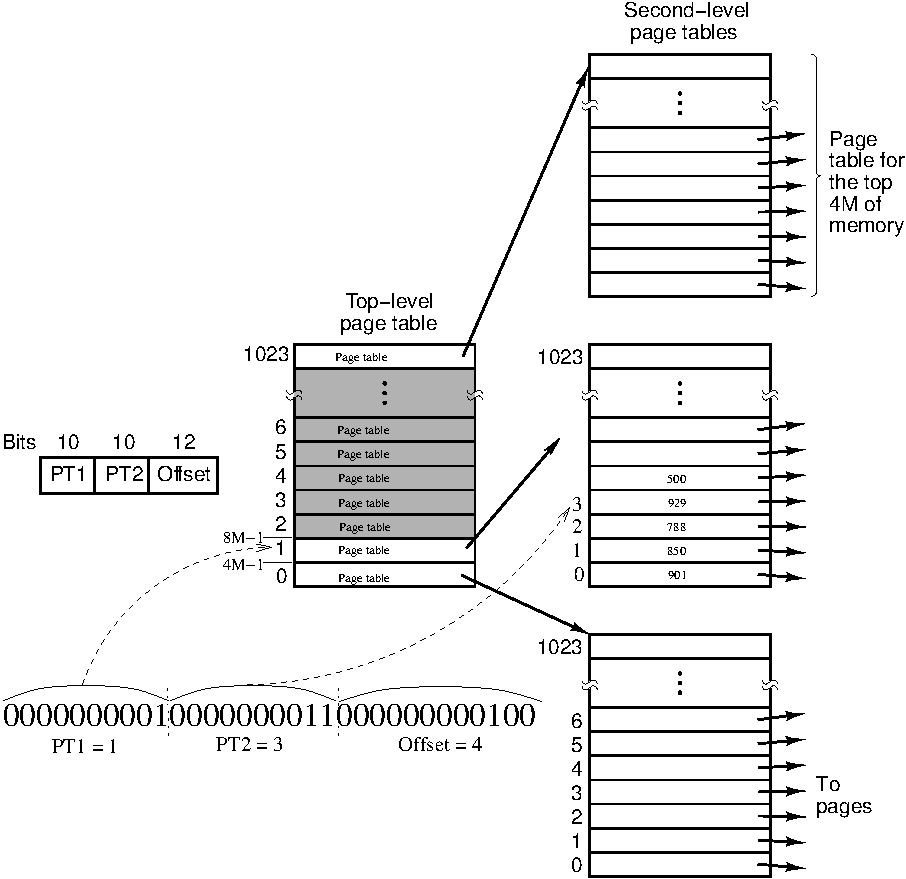
\includegraphics[width=\paperwidth]{mos-figs-4-12}};

  \begin{scope}[x={(image.south east)},y={(image.north west)}]%
    % %%% grid
    % \draw[help lines,xstep=.1,ystep=.1] (0,0) grid (1,1);%
    % \foreach \x in {0,1,...,9} { \node [xy,anchor=north] at (\x/10,0) {0.\x}; }%
    % \foreach \y in {0,1,...,9} { \node [xy,anchor=east] at (0,\y/10) {0.\y}; }%

    \node at (.05,.6) [anchor=south west,blue!50] {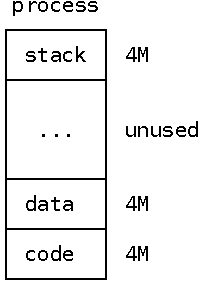
\includegraphics[scale=1.5]{process}};
  \end{scope}

\end{tikzpicture}}
  \caption{Two-level paging}
  \label{fig:2-level-paging-big}
\end{figure}

\tikzsetnextfilename{mm-seg}
\begin{figure}
  \centering\resizebox{\textwidth}{!}{
\begin{tikzpicture}[every node/.style = {inner sep=0}]
  
  %%% background image
  \node[anchor=south west] (image) at (0,0)%
  {\includegraphics[width=\paperwidth]{osc-8-46}};

  \begin{scope}[x={(image.south east)},y={(image.north west)}]%
    %%% grid
    % \draw[help lines,xstep=.1,ystep=.1] (0,0) grid (1,1);%
    % \foreach \x in {0,1,...,9} { \node [xy,anchor=north] at (\x/10,0) {0.\x}; }%
    % \foreach \y in {0,1,...,9} { \node [xy,anchor=east] at (0,\y/10) {0.\y}; }%

    \node at (.6,.54) [color=gray,scale=8] {\ding{224}};
  \end{scope}
\end{tikzpicture}}
  \caption{Memory segmentation}
  \label{fig:mm-seg}
\end{figure}

\tikzsetnextfilename{seg-trans}
\begin{figure}
  \centering\resizebox{\textwidth}{!}{
\begin{tikzpicture}[node distance=5pt,%
  every node/.style = {inner sep=0,align=center},%
  ]
  
  %%% background image
  \node[anchor=south west] (image) at (0,0)%
  {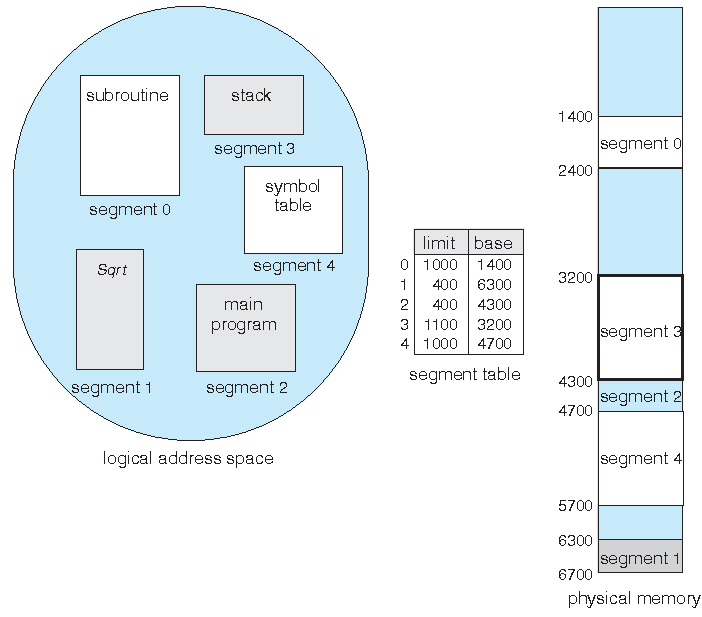
\includegraphics[width=\paperwidth]{osc-8-50}};

  % http://tex.stackexchange.com/questions/9559/drawing-on-an-image-with-tikz
  \begin{scope}[x={(image.south east)},y={(image.north west)}]%
    %%% grid
    % \draw[help lines,xstep=.1,ystep=.1] (0,0) grid (1,1);%
    % \foreach \x in {0,1,...,9} { \node [xy,anchor=north] at (\x/10,0) {0.\x}; }%
    % \foreach \y in {0,1,...,9} { \node [xy,anchor=east] at (0,\y/10) {0.\y}; }%

    \node at (.07,.17) [anchor=north west,scale=2,blue!70] {%
      $(2,53)\Rightarrow{}4300+53=4353$\\
      $(3,852)\Rightarrow{}3200+852=4052$\\
      $(0,1222)\Rightarrow{}\,\text{Trap!}$};
  \end{scope}
\end{tikzpicture}}
  \caption{Memory segmentation --- Address translation}
  \label{fig:seg-trans}
\end{figure}

\tikzsetnextfilename{fs-tables}
\begin{figure}
  \centering
  \begin{tikzpicture}[%
    decoration={amplitude=1.5pt}, penciline={jag ratio=1.5},%
    ultra thick,font=\fontspec{Humor Sans},%
    table node/.style={rectangle split, rectangle split parts=#1, decorate, draw, anchor=center},
    arrow/.style = {decorate,->,dashed,gray!90,draw}]%    

    \node (ufdt) [table node=4, minimum width=1.8cm, %
    label={above, align=center:{User\\File Descriptor\\Table}}] %
    {\rule{0pt}{7mm}%
      \nodepart{two}\rule{0pt}{7mm}%
      \nodepart{three}\rule{0pt}{7mm}%
      \nodepart{four}\rule{0pt}{4cm}};

    \node (ft) [table node=5, minimum width=8mm,
    label={above, align=center:{File\\Table}},%
    right=3cm of ufdt.north east, anchor=north west]%
    {\rule{0pt}{2cm}%
      \nodepart{two}\rule{0pt}{7mm}%
      \nodepart{three}\rule{0pt}{1.5cm}%
      \nodepart{four}\rule{0pt}{7mm}%
      \nodepart{five}\rule{0pt}{1.5cm}};
    
    \node (it) [table node=5, minimum width=8mm,
    label={above, align=center:{Inode\\Table}},%
    right=4cm of ft.north east, anchor=north west]%
    {\rule{0pt}{1.5cm}%
      \nodepart{two}\rule{0pt}{7mm}%
      \nodepart{three}\rule{0pt}{1.5cm}%
      \nodepart{four}\rule{0pt}{7mm}%
      \nodepart{five}\rule{0pt}{2cm}};

    \draw [arrow] (ufdt.text east) -- (ft.two west);%
    \draw [arrow] (ufdt.two east) -- (ft.two west);%
    \draw [arrow] (ufdt.three east) -- (ft.four west);%
    \draw [arrow] (ft.two east) -- (it.two west);%
    \draw [arrow] (ft.four east) -- (it.four west);

\end{tikzpicture}  
  \caption{File system tables}
  \label{fig:fs-tables}
\end{figure}

\tikzsetnextfilename{file-tables2}
\begin{figure}
  \centering
\begin{tikzpicture}[decoration={amplitude=2pt}, penciline={jag ratio=2},%
  font=\fontspec{Humor Sans}, thick, align=center,%
  arrow/.style = {->,dashed,decorate},%
  table node/.style={rectangle split, rectangle split parts=#1, decorate, draw, anchor=center}]%  

  \node (fdt) [table node=7,%
  label={above,align=center:{User\\File Descriptor\\Table}}]%
  { STDIN \nodepart{two} STDOUT \nodepart{three} STDERR \nodepart{four} /etc/passwd \nodepart{five}
    local \nodepart{six} /etc/passwd \nodepart{seven} \vdots };%

  \node at ($(fdt.text west)+(-5pt,0)$) {0};%
  \node at ($(fdt.two west)+(-5pt,0)$) {1};%
  \node at ($(fdt.three west)+(-5pt,0)$) {2};%
  \node at ($(fdt.four west)+(-5pt,0)$) {3};%
  \node at ($(fdt.five west)+(-5pt,0)$) {4};%
  \node at ($(fdt.six west)+(-5pt,0)$) {5};%
  \node at ($(fdt.seven west)+(-5pt,0)$) {\vdots};%
  
  \node (ft) [table node=6, right=of fdt.north east,anchor=north west,%
  label={above,align=center:{Global\\Open File\\Table}}]%
  { \vdots \nodepart{two} count 1\\R \nodepart{three} \vdots \nodepart{four} count 1\\RW
    \nodepart{five} \vdots \nodepart{six} count 1\\W };%

  \node (it) [table node=5, right=of ft.north east,anchor=north west,%
  label={above,align=center:{Inode\\Table}}]%
  { \vdots\\\vdots\\\vdots \nodepart{two} (/etc/passwd)\\count 2 \nodepart{three} \vdots
    \nodepart{four} (local)\\count 1 \nodepart{five} \vdots };%

  \draw [arrow] (fdt.four east)--(ft.two west);%
  \draw [arrow] (fdt.five east)--(ft.four west);%
  \draw [arrow] (fdt.six east)--(ft.six west);%

  \draw [arrow] (ft.two east)--(it.two west);%
  \draw [arrow] (ft.four east)--(it.four west);%
  \draw [arrow] (ft.six east)--(it.two west);%
\end{tikzpicture}  
  \caption{File tables}
  \label{fig:file-tables2}
\end{figure}

\tikzsetnextfilename{file-tables3}
\begin{figure}
  \centering
\begin{tikzpicture}[ decoration={amplitude=2pt}, penciline={jag ratio=2},%
  font=\fontspec{Humor Sans}, thick, align=center,%
  arrow/.style = {->,dashed,decorate},%
  table node/.style={rectangle split, rectangle split parts=#1, decorate, draw, anchor=center}] 

  \node (fdt) [table node=7,%
  label={above:{{\scriptsize Proc A}}},%
  label={above,yshift=4ex,align=center:{User\\File Descriptor\\Table}}]%
  { STDIN \nodepart{two} STDOUT \nodepart{three} STDERR \nodepart{four} /etc/passwd \nodepart{five}
    local \nodepart{six} /etc/passwd \nodepart{seven} \vdots};

  \node at ($(fdt.text west)+(-5pt,0)$) {0};%
  \node at ($(fdt.two west)+(-5pt,0)$) {1};%
  \node at ($(fdt.three west)+(-5pt,0)$) {2};%
  \node at ($(fdt.four west)+(-5pt,0)$) {3};%
  \node at ($(fdt.five west)+(-5pt,0)$) {4};%
  \node at ($(fdt.six west)+(-5pt,0)$) {5};%
  \node at ($(fdt.seven west)+(-5pt,0)$) {\vdots};%

  \node (ft) [table node=10,%
  right=3cm of fdt.north east,anchor=north west,%
  label={above,align=center:{Global\\Open File\\Table}}]%
  { \vdots \nodepart{two} count 1\\R \nodepart{three} \vdots \nodepart{four} count 1\\RW
    \nodepart{five} \vdots \nodepart{six} count 1\\R \nodepart{seven} \vdots
    \nodepart{eight} count 1\\W \nodepart{nine} \vdots \nodepart{ten} count 1\\R};

  \draw [arrow] (fdt.four east)--(ft.two west);%
  \draw [arrow] (fdt.five east)--(ft.four west);%
  \draw [arrow] (fdt.six east)--(ft.eight west);%

  \node (it) [table node=7,%
  right=3cm of ft.north east,anchor=north west,%
  label={above,align=center:{Inode Table}}]%
  {
    \vdots\\\vdots
    \nodepart{two} (/etc/passwd)\\count 3
    \nodepart{three} \vdots\\\vdots
    \nodepart{four} (local)\\count 1
    \nodepart{five} \vdots\\\vdots
    \nodepart{six} (private)\\count 1
    \nodepart{seven} \vdots\\\vdots   
  };

  \draw [arrow] (ft.two east)--(it.two west);%
  \draw [arrow] (ft.four east)--(it.four west);%
  \draw [arrow] (ft.six east)--(it.two west);%
  \draw [arrow] (ft.eight east)--(it.two west);%
  \draw [arrow] (ft.ten east)--(it.six west);%

  \node (fdtb) [table node=6, below=of fdt.south,anchor=north,%
  label={above:{{\scriptsize Proc B}}}]%
  { STDIN \nodepart{two} STDOUT \nodepart{three} STDERR \nodepart{four} /etc/passwd \nodepart{five}
    private \nodepart{six} \vdots };

  \draw [arrow] (fdtb.four east)-- (ft.six west);%
  \draw [arrow] (fdtb.five east)-- (ft.ten west);%  
\end{tikzpicture}  
  \caption{File tables}
  \label{fig:file-tables3}
\end{figure}

\tikzsetnextfilename{vfs-objs}
\begin{figure}
  \centering
  \begin{tikzpicture}[%
    list/.style={rectangle split, rectangle split horizontal,%
      rectangle split parts=5, draw},%
    thick,%
    arrow/.style={thick,->},%
    squarebox/.style={draw,align=center,minimum width=2.2cm,minimum height=1cm,fill=blue!20},%
    dentrybox/.style={draw,align=center,minimum height=1cm,fill=red!20},%
    cylinderbox/.style={draw,%
      cylinder,shape border rotate=90,aspect=.25,%
      cylinder uses custom fill,%
      cylinder body fill=gray!10, cylinder end fill=gray!30,%
      minimum width=1.5cm,minimum height=2cm,align=center},%
  ] 

  \node (p1) [squarebox] {Process 1};%
  \node (p2) [squarebox,below=of p1,yshift=.8cm] {Process 2};%
  \node (p3) [squarebox,below=of p2,yshift=.8cm] {Process 3};%

  \node (f1) [squarebox,right=of p1] {File object};%
  \node (f2) [squarebox,right=of p2] {File object};%
  \node (f3) [squarebox,right=of p3] {File object};%

  \node (dentry) [dentrybox,list,right=of f2.east] {%
    \nodepart{one}\nodepart{three}\nodepart{five}%
    \nodepart{two}dentry\\object%
    \nodepart{four}dentry\\object};%
  
  \node (inode) [squarebox,fill=brown!20,above=2cm of dentry.four north] {inode\\object};%

  \node (sb) [squarebox,fill=violet!20,left=of inode] {Superblock\\object};%

  \node (disk) [cylinderbox,left=of sb.south west,anchor=south east] {disk\\file};%

  \path%
  (p1) edge [arrow, "fd"] (f1)%
  (p2) edge [arrow] (f2)%
  (p3) edge [arrow] (f3);

  \draw [arrow,dashed] (f1.east) -| node [above,xshift=-.7cm,scale=.6] {f\_dentry}%
  (dentry.one split north);
  
  \draw [arrow,dashed] (f2.east) -- ($(f2.east) + (.3cm,0)$) |- %
  ($(dentry.west) + (0,-.9cm)$) -| (dentry.one split south);%
  
  \draw [arrow,dashed] (f3.east) -| (dentry.three split south);
  
  \draw [arrow,dotted] (dentry.two north) |- ($(inode.south west) + (.5cm,-1cm)$)%
  -| node [above,xshift=-.7cm,scale=.6] {d\_inode} ($(inode.south west) + (.5cm,0)$);%

  \draw [arrow,dotted] (dentry.four north) -- (inode);%
  \draw [arrow] (inode) -- node [above,scale=.6] {i\_sb} (sb);%
  \draw [arrow,dotted] (sb) -- (disk.-13);
  \draw [arrow,dotted] (inode.north) |- ($(disk.east) + (0,.7cm)$);
\end{tikzpicture}  
  \caption{VFS objects}
  \label{fig:vfs-objs}
\end{figure}

\tikzsetnextfilename{vfs-objs-bw}
\begin{figure}
  \centering
  \begin{tikzpicture}[%
    list/.style={rectangle split, rectangle split horizontal,%
      rectangle split parts=5, draw},%
    thick,%
    arrow/.style={thick,->},%
    squarebox/.style={draw,align=center,minimum width=2.2cm,minimum height=1cm},%
    dentrybox/.style={draw,align=center,minimum height=1cm},%
    cylinderbox/.style={draw,%
      cylinder,shape border rotate=90,aspect=.25,%
      cylinder uses custom fill,%
      cylinder body fill=gray!10, cylinder end fill=gray!30,%
      minimum width=1.5cm,minimum height=2cm,align=center},%
  ] 

  \node (p1) [squarebox] {Process 1};%
  \node (p2) [squarebox,below=of p1,yshift=.8cm] {Process 2};%
  \node (p3) [squarebox,below=of p2,yshift=.8cm] {Process 3};%

  \node (f1) [squarebox,right=of p1] {File object};%
  \node (f2) [squarebox,right=of p2] {File object};%
  \node (f3) [squarebox,right=of p3] {File object};%

  \node (dentry) [dentrybox,list,right=of f2.east] {%
    \nodepart{one}\nodepart{three}\nodepart{five}%
    \nodepart{two}dentry\\object%
    \nodepart{four}dentry\\object};%
  
  \node (inode) [squarebox,above=2cm of dentry.four north] {inode\\object};%

  \node (sb) [squarebox,left=of inode] {Superblock\\object};%

  \node (disk) [cylinderbox,left=of sb.south west,anchor=south east] {disk\\file};%

  \path%
  (p1) edge [arrow, "fd"] (f1)%
  (p2) edge [arrow] (f2)%
  (p3) edge [arrow] (f3);

  \draw [arrow,dashed] (f1.east) -| node [above,xshift=-.7cm,scale=.6] {f\_dentry}%
  (dentry.one split north);
  
  \draw [arrow,dashed] (f2.east) -- ($(f2.east) + (.3cm,0)$) |- %
  ($(dentry.west) + (0,-.9cm)$) -| (dentry.one split south);%
  
  \draw [arrow,dashed] (f3.east) -| (dentry.three split south);
  
  \draw [arrow,dotted] (dentry.two north) |- ($(inode.south west) + (.5cm,-1cm)$)%
  -| node [above,xshift=-.7cm,scale=.6] {d\_inode} ($(inode.south west) + (.5cm,0)$);%

  \draw [arrow,dotted] (dentry.four north) -- (inode);%
  \draw [arrow] (inode) -- node [above,scale=.6] {i\_sb} (sb);%
  \draw [arrow,dotted] (sb) -- (disk.-13);
  \draw [arrow,dotted] (inode.north) |- ($(disk.east) + (0,.7cm)$);
\end{tikzpicture}  
  \caption{VFS objects}
  \label{fig:vfs-objs-bw}
\end{figure}

\tikzsetnextfilename{vfs-cp}
\begin{figure}
  \centering
\begin{tikzpicture}[%
  %decoration={random steps,segment length=3pt,amplitude=.3pt},%
  thick,node distance=0pt,%
  roundbox/.style ={ellipse,fill=blue!20,inner sep=1pt,minimum width=1.5cm},%
  squarebox/.style ={fill=orange!30,minimum width=3cm},%
  cylinderbox/.style ={cylinder,shape border rotate=90,aspect=.25,%
    cylinder uses custom fill,%
    cylinder body fill=black!30, cylinder end fill=black!50,%
    minimum width=1.5cm,inner sep=1pt},%minimum height=1cm,},%
  arrowbox/.style ={double arrow,rotate=90,scale=.7,fill=gray!50,%
    inner xsep=.5cm,inner ysep=.5cm,%
    double arrow tip angle=135,%
    double arrow head extend=6pt},%
  every node/.style ={draw}%decorate,
  ] 

  \node (cp) [roundbox] {cp};%
  \node (arrow1) [arrowbox,below=of cp.south,anchor=east] {};%
  \node (vfs) [squarebox,below=of arrow1.west,anchor=north] {VFS};%
  \node (arrow2) [arrowbox,below=of vfs.south west,anchor=east,yshift=-5ex] {};%
  \node (arrow3) [arrowbox,below=of vfs.south east,anchor=east,yshift=5ex] {};%
  \node (ext2) [cylinderbox,below=of arrow2.west,anchor=north] {ext2};%
  \node (dos)  [cylinderbox,below=of arrow3.west,anchor=north,scale=.8] {MS-DOS};%
  \node (test1) [draw=none,below=1ex of ext2,scale=.5] {/tmp/test};%
  \node (test2) [draw=none,below=1ex of dos,scale=.5] {/floppy/TEST};%

\end{tikzpicture}  
  \caption{VFS file copy}
  \label{fig:vfs-cp}
\end{figure}

\tikzsetnextfilename{vfs-cp-bw}
\begin{figure}
  \centering
\begin{tikzpicture}[%
  %decoration={random steps,segment length=3pt,amplitude=.3pt},%
  thick,node distance=0pt,%
  roundbox/.style ={ellipse,inner sep=1pt,minimum width=1.5cm},%
  squarebox/.style ={minimum width=3cm},%
  cylinderbox/.style ={cylinder,shape border rotate=90,aspect=.25,%
    minimum width=1.5cm,inner sep=1pt},%minimum height=1cm,},%
  arrowbox/.style ={double arrow,rotate=90,scale=.7,%
    inner xsep=.5cm,inner ysep=.5cm,%
    double arrow tip angle=135,%
    double arrow head extend=6pt},%
  every node/.style ={draw}%%decorate,
  ] 

  \node (cp) [roundbox] {cp};%
  \node (arrow1) [arrowbox,below=of cp.south,anchor=east] {};%
  \node (vfs) [squarebox,below=of arrow1.west,anchor=north] {VFS};%
  \node (arrow2) [arrowbox,below=of vfs.south west,anchor=east,yshift=-5ex] {};%
  \node (arrow3) [arrowbox,below=of vfs.south east,anchor=east,yshift=5ex] {};%
  \node (ext2) [cylinderbox,below=of arrow2.west,anchor=north] {ext2};%
  \node (dos)  [cylinderbox,below=of arrow3.west,anchor=north,scale=.8] {MS-DOS};%
  \node (test1) [draw=none,below=1ex of ext2,scale=.5] {/tmp/test};%
  \node (test2) [draw=none,below=1ex of dos,scale=.5] {/floppy/TEST};%

\end{tikzpicture}  
  \caption{VFS file copy (bw version)}
  \label{fig:vfs-cp-bw}
\end{figure}

\tikzsetnextfilename{dma-handshaking}
\begin{figure}
  \centering
\begin{tikzpicture}
  \begin{umlseqdiag}
    \umlobject[class=]{Disk}
    \umlobject[class=]{Disk Controller}
    \umlobject[class=]{DMA Controller}
    \umlobject[class=]{Memory}
    % \umlobject[class=Register, fill=blue!20]{status}
    % \umlobject[class=Register, fill=blue!20]{control}
    % \umlobject[class=Register, fill=blue!20]{data-out}
    % \umlobject[class=]{Controller}
    \begin{umlcall}[op={read},return=data]{Disk Controller}{Disk}
    \end{umlcall}
    \begin{umlcallself}[op={data ready?},return=yes]{Disk Controller}
    \end{umlcallself}
    \begin{umlcall}[op={DMA\emph{-request}}]{Disk Controller}{DMA Controller}
    \end{umlcall}
    \begin{umlcall}[op={memory address}]{DMA Controller}{Disk Controller}
      \begin{umlcall}[op={DMA\emph{-acknowledge}}]{DMA Controller}{Disk Controller}          
      \end{umlcall}
    \end{umlcall}
    \begin{umlcall}[op={data}]{Disk Controller}{Memory}        
    \end{umlcall}
  \end{umlseqdiag}
\end{tikzpicture}
  \caption{DMA handshaking}
  \label{fig:dma-handshaking}
\end{figure}

\tikzsetnextfilename{handshaking}
\begin{figure}
  \centering
\begin{tikzpicture}
  \begin{umlseqdiag}
    \umlobject[class=]{Host}
    \umlobject[class=Register, fill=blue!20]{status}
    \umlobject[class=Register, fill=blue!20]{control}
    \umlobject[class=Register, fill=blue!20]{data-out}
    \umlobject[class=]{Controller}
    \begin{umlcall}[op={\emph{busy} = ?},fill=red!10, return=0]{Host}{status}
    \end{umlcall}
    \begin{umlcall}[op=write a byte]{Host}{data-out}
    \end{umlcall}
    \begin{umlcall}[op={\emph{command-ready} = 1}]{Host}{status}
    \end{umlcall}
    \begin{umlcall}[dt=18, op={\emph{command-ready} = ?}, return=1]{Controller}{status}
    \end{umlcall}
    \begin{umlcall}[dt=5,op={\emph{busy} = 1}]{Controller}{status}        
    \end{umlcall}
    \begin{umlcall}[op={\emph{write} == 1?}, return=1]{Controller}{control}        
    \end{umlcall}
    \begin{umlcall}[dt=4,op=read, return=1 byte]{Controller}{data-out}
    \end{umlcall}
    \begin{umlcall}[dt=5,op={\emph{command-ready} = 0, \emph{error} = 0, \emph{busy} = 0}]{Controller}{status}        
    \end{umlcall}
  \end{umlseqdiag}
\end{tikzpicture}
  \caption{Handshaking}
  \label{fig:handshaking}
\end{figure}

\end{document}
%%% Local Variables:
%%% mode: latex
%%% TeX-master: t
%%% End:
